% !TeX root = ../main.tex

\appendix

\chapter{Aanvullende afbeeldingen}
% !TeX root = ../main.tex

% These appendix images are intentionally placed in a fixed grid instead of separate floating
% figures. Separate floats made LaTeX move almost every screenshot to its own page, while this
% layout keeps the appendix compact and still preserves the figure labels used in the text.
\begin{center}
  \begin{minipage}[t]{0.48\textwidth}
    \centering
    \refstepcounter{figure}\label{fig:timingdata1}
    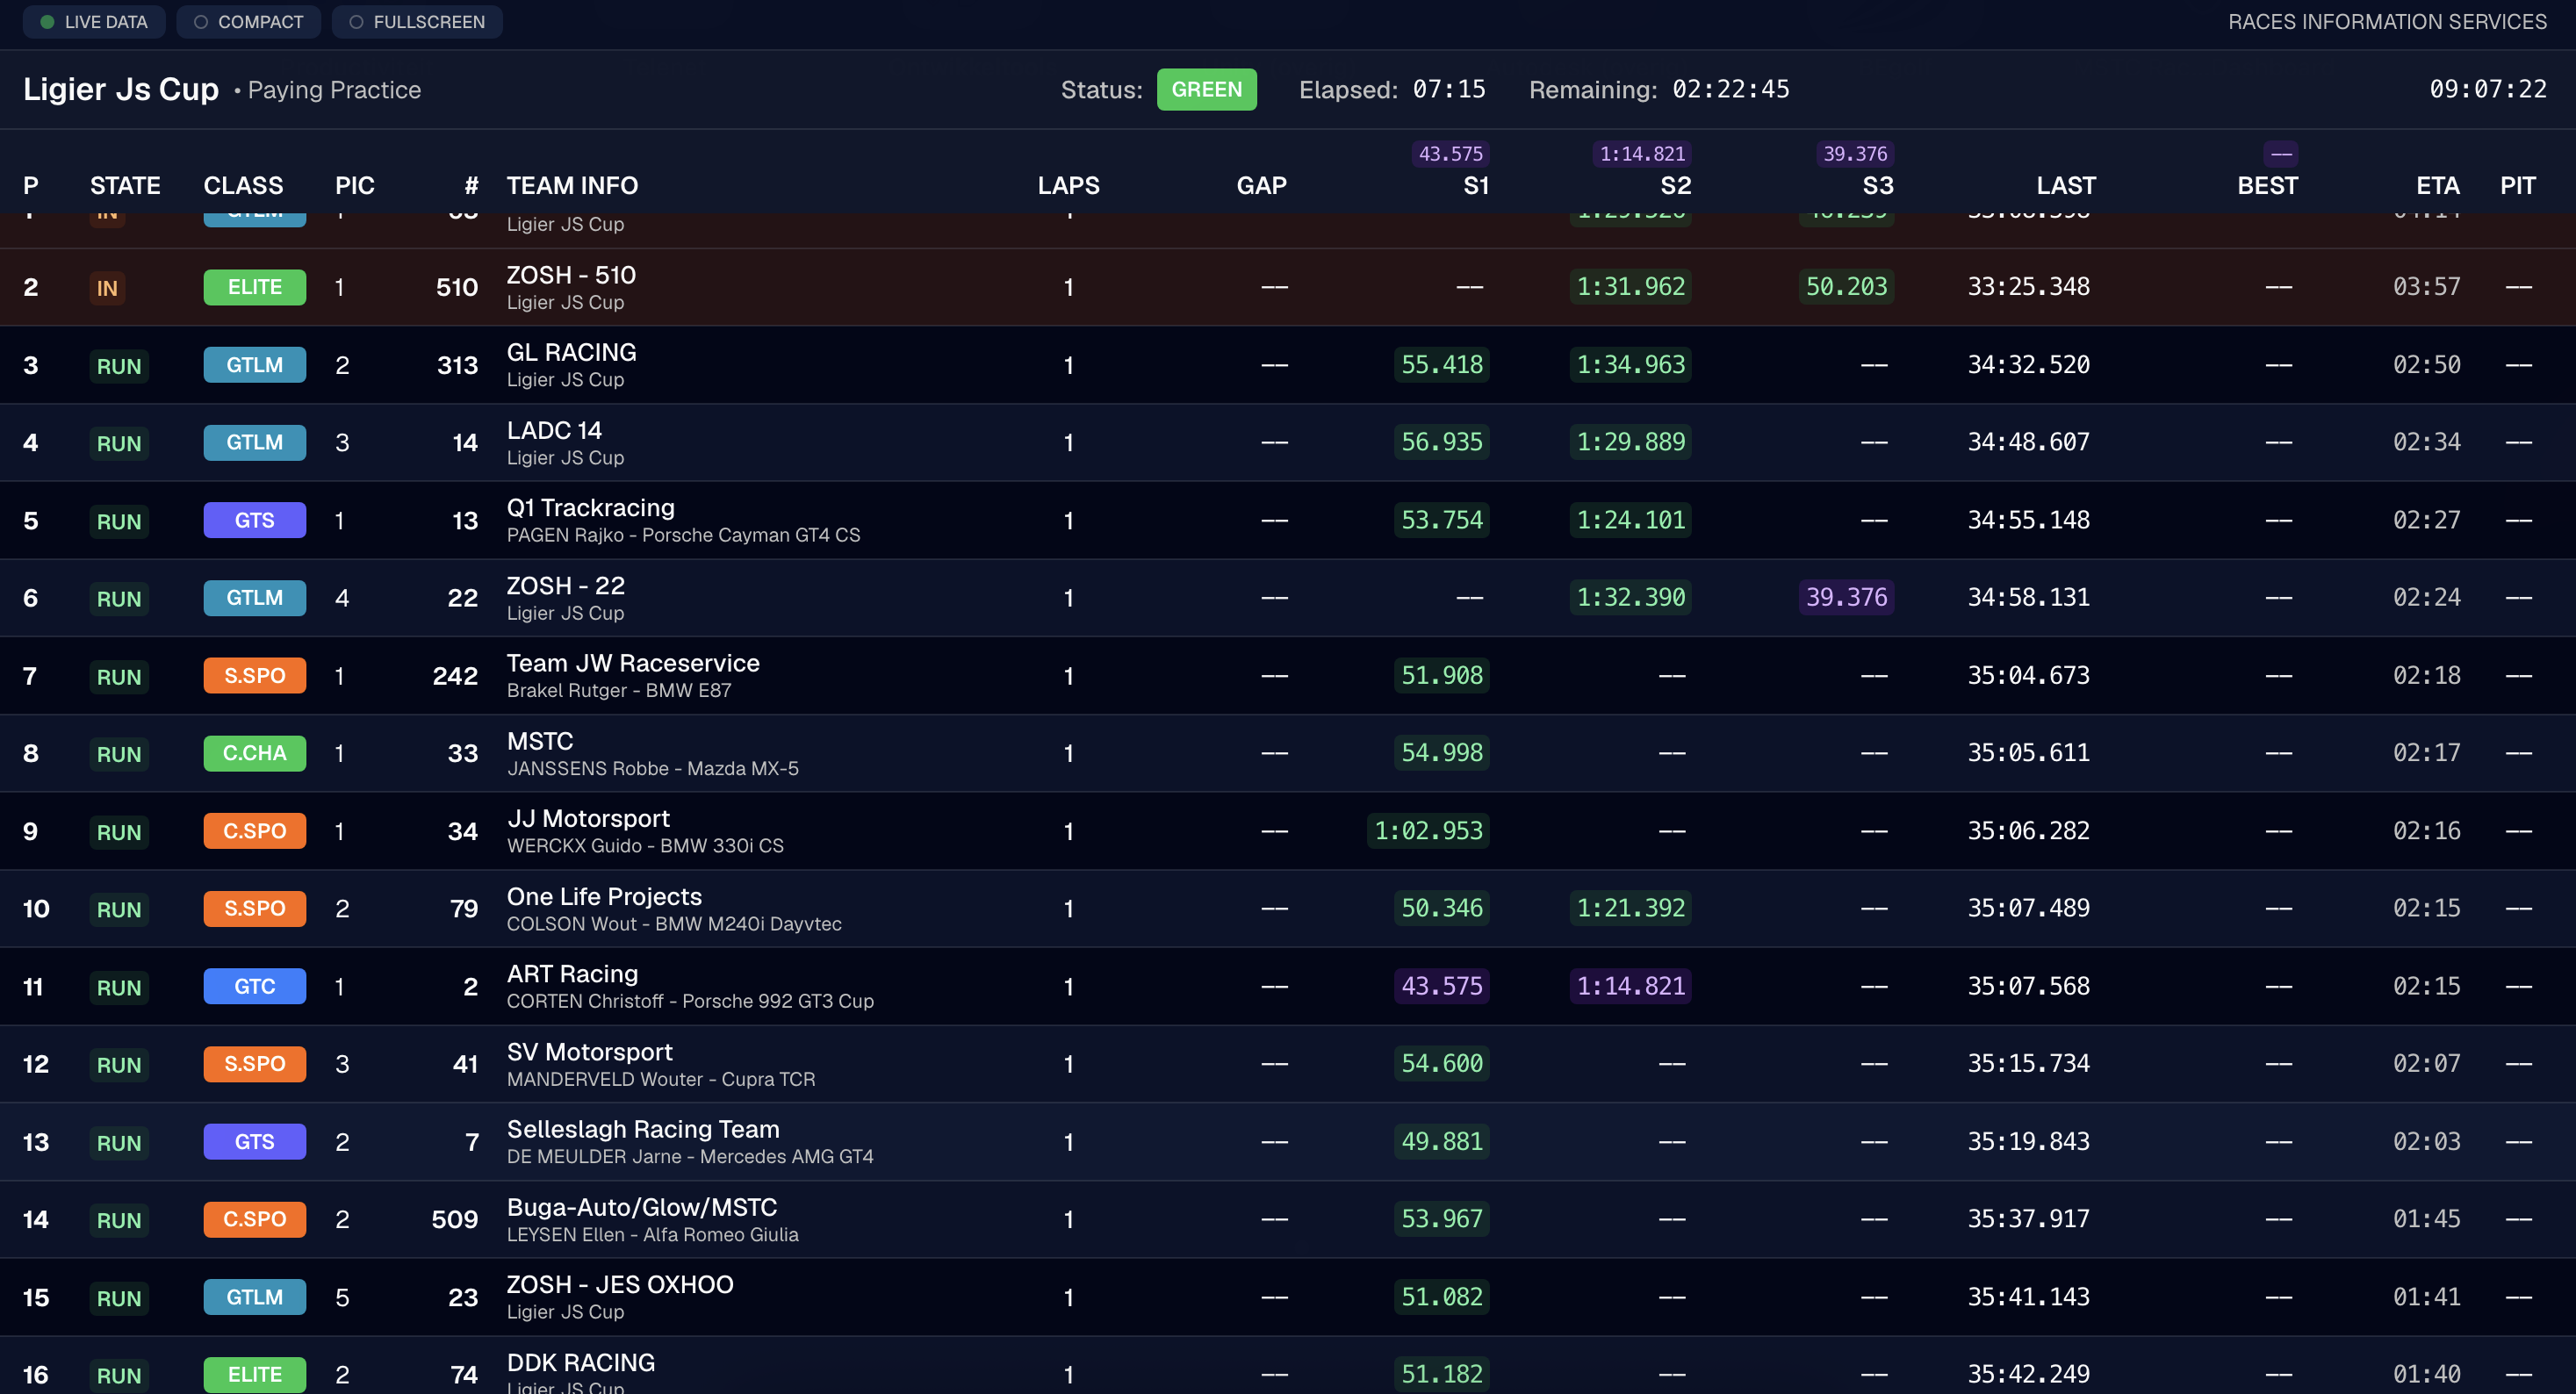
\includegraphics[width=\linewidth]{../figures/timingdata1.png}

    \small\textbf{Figuur~\thefigure:} Screenshot van de officiële timingpagina tijdens de race in
    Spa-Francorchamps. De tabel toont actuele ronde- en sectortijden en maakt zichtbaar hoe
    verschillende klassen door elkaar staan.
  \end{minipage}\hfill
  \begin{minipage}[t]{0.48\textwidth}
    \centering
    \refstepcounter{figure}\label{fig:dashboard-schets1}
    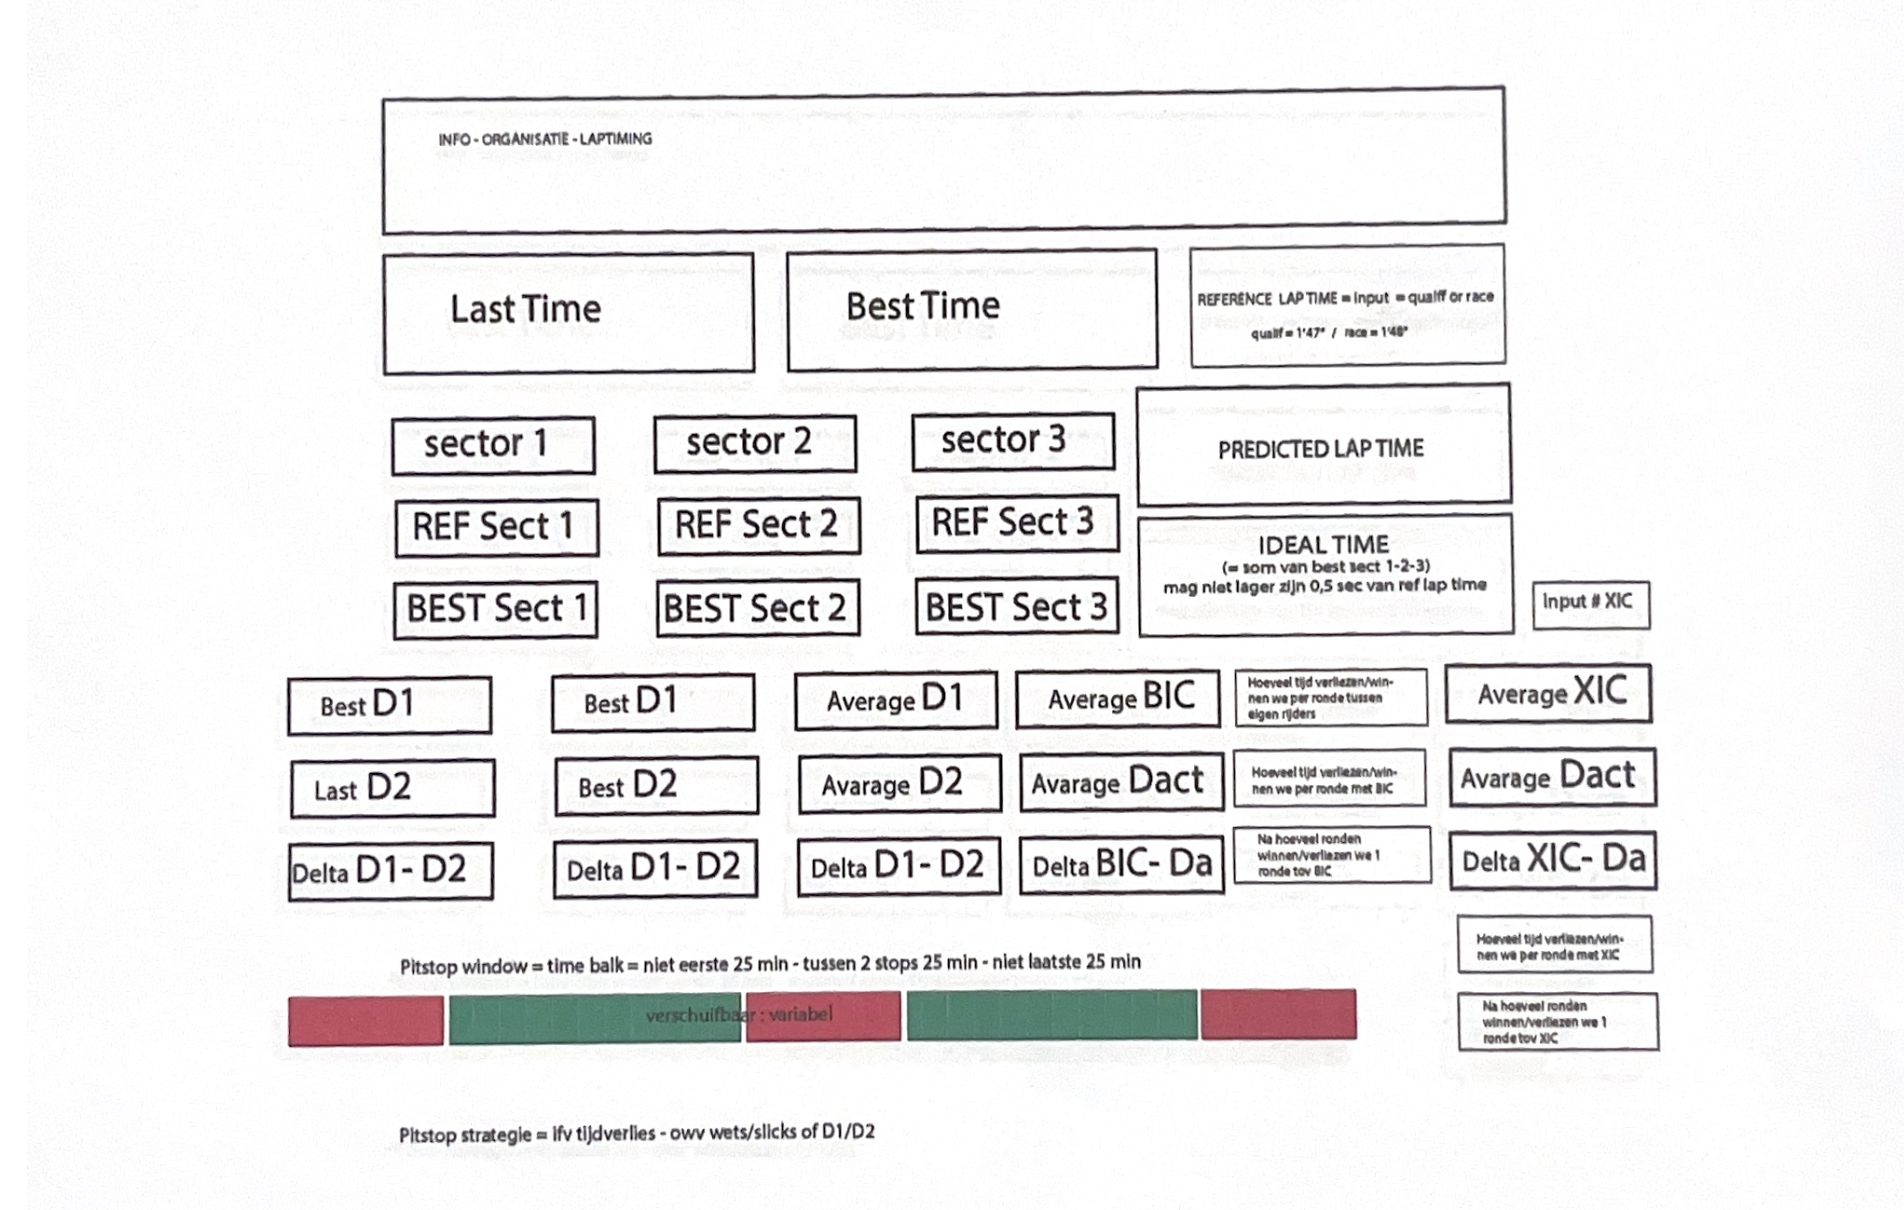
\includegraphics[width=\linewidth]{../figures/dashboard-schets1.png}

    \small\textbf{Figuur~\thefigure:} Schets van het eerste dashboardontwerp. Deze schets werd door
    de opdrachtgever gemaakt en vormde de basis voor de eerste werkende versie.
  \end{minipage}

  \vspace{1.2em}

  \begin{minipage}[t]{0.48\textwidth}
    \centering
    \refstepcounter{figure}\label{fig:versie1}
    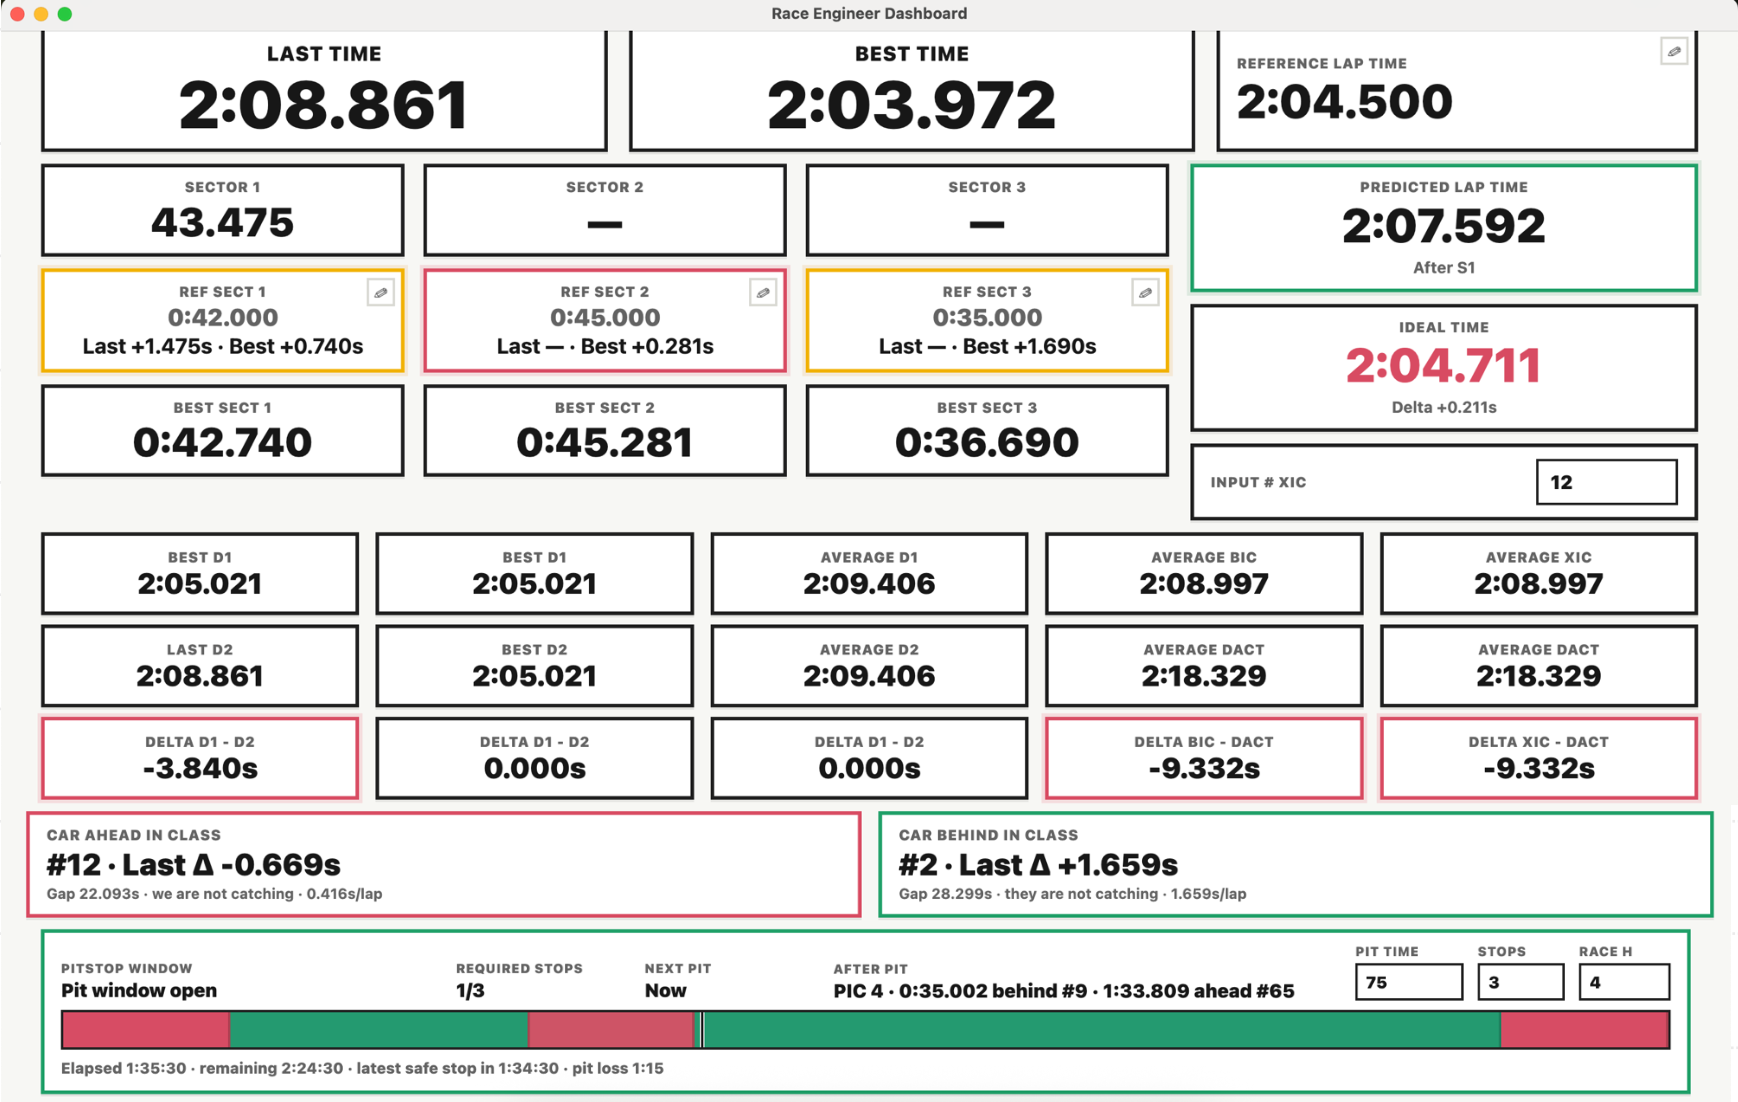
\includegraphics[width=\linewidth]{../figures/versie1.png}

    \small\textbf{Figuur~\thefigure:} Eerste werkende versie van het dashboard, getest tijdens de
    race in Spa-Francorchamps.
  \end{minipage}\hfill
  \begin{minipage}[t]{0.48\textwidth}
    \centering
    \refstepcounter{figure}\label{fig:grafiekvenster1}
    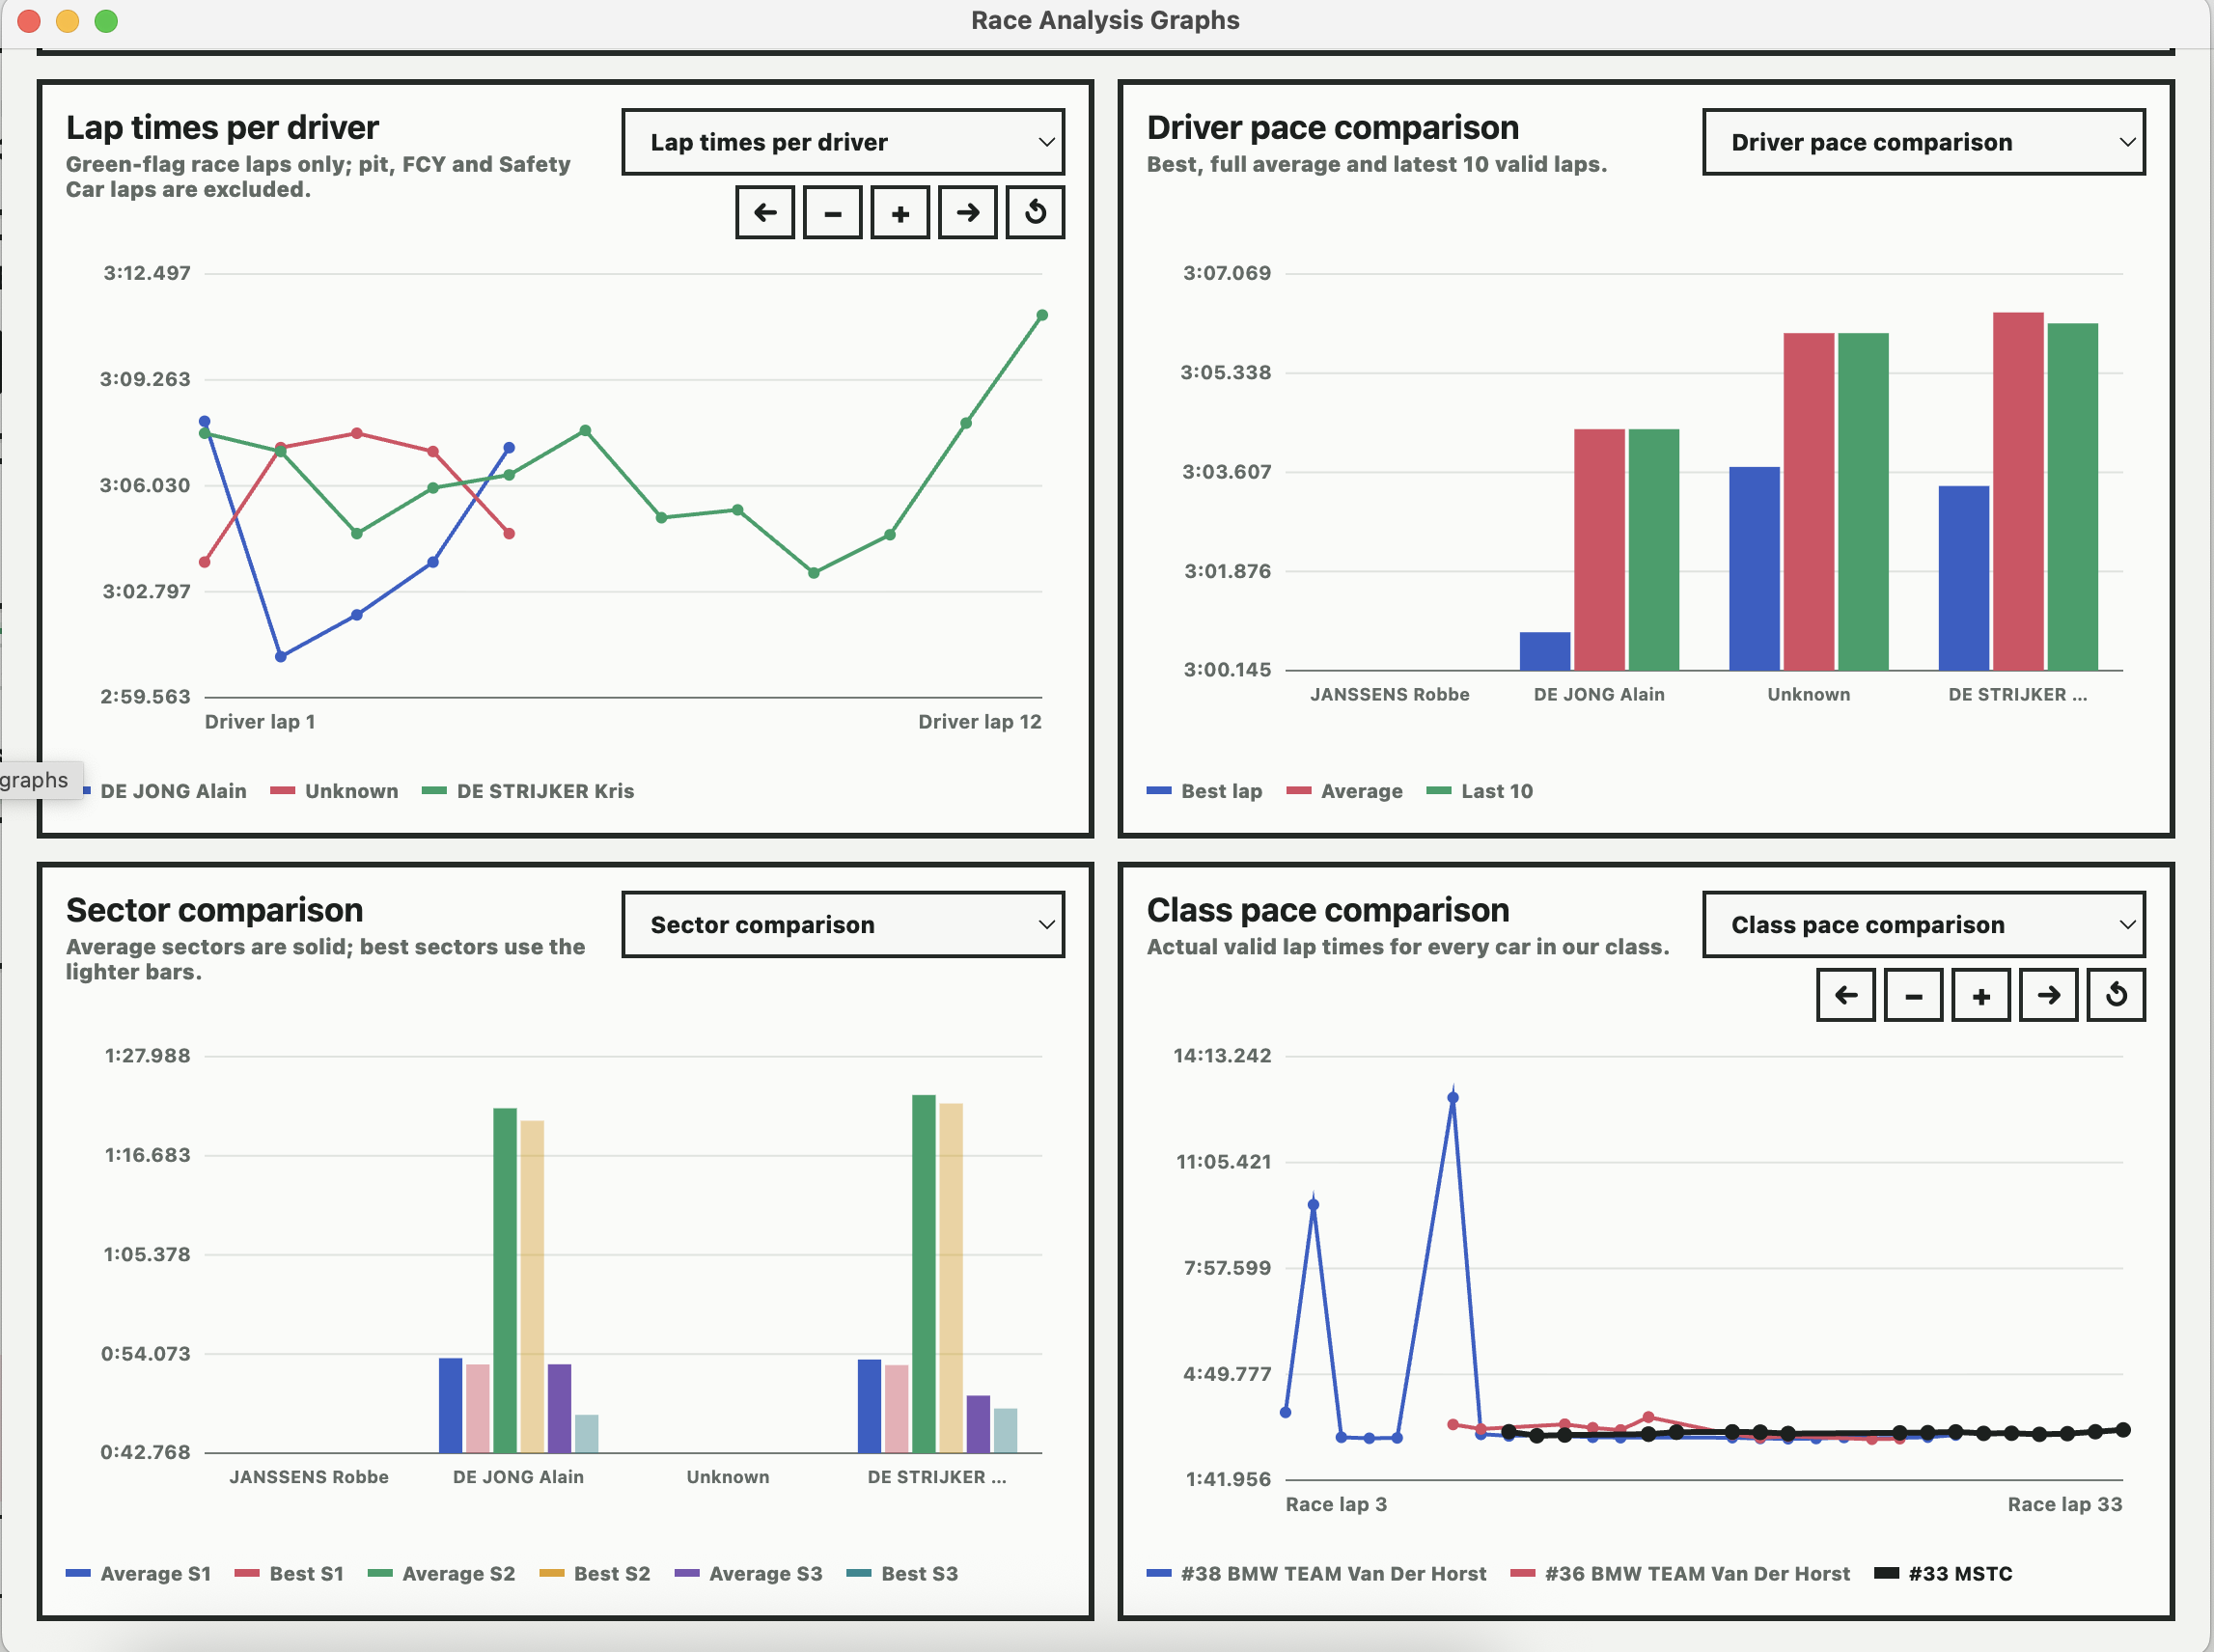
\includegraphics[width=\linewidth]{../figures/grafiekvenster1.png}

    \small\textbf{Figuur~\thefigure:} Eerste werkende grafiekenvenster waarin de evolutie van
    rondetijden en sectoren visueel wordt weergegeven.
  \end{minipage}

  \vspace{1.2em}

  \begin{minipage}[t]{0.48\textwidth}
    \centering
    \refstepcounter{figure}\label{fig:versie1}
    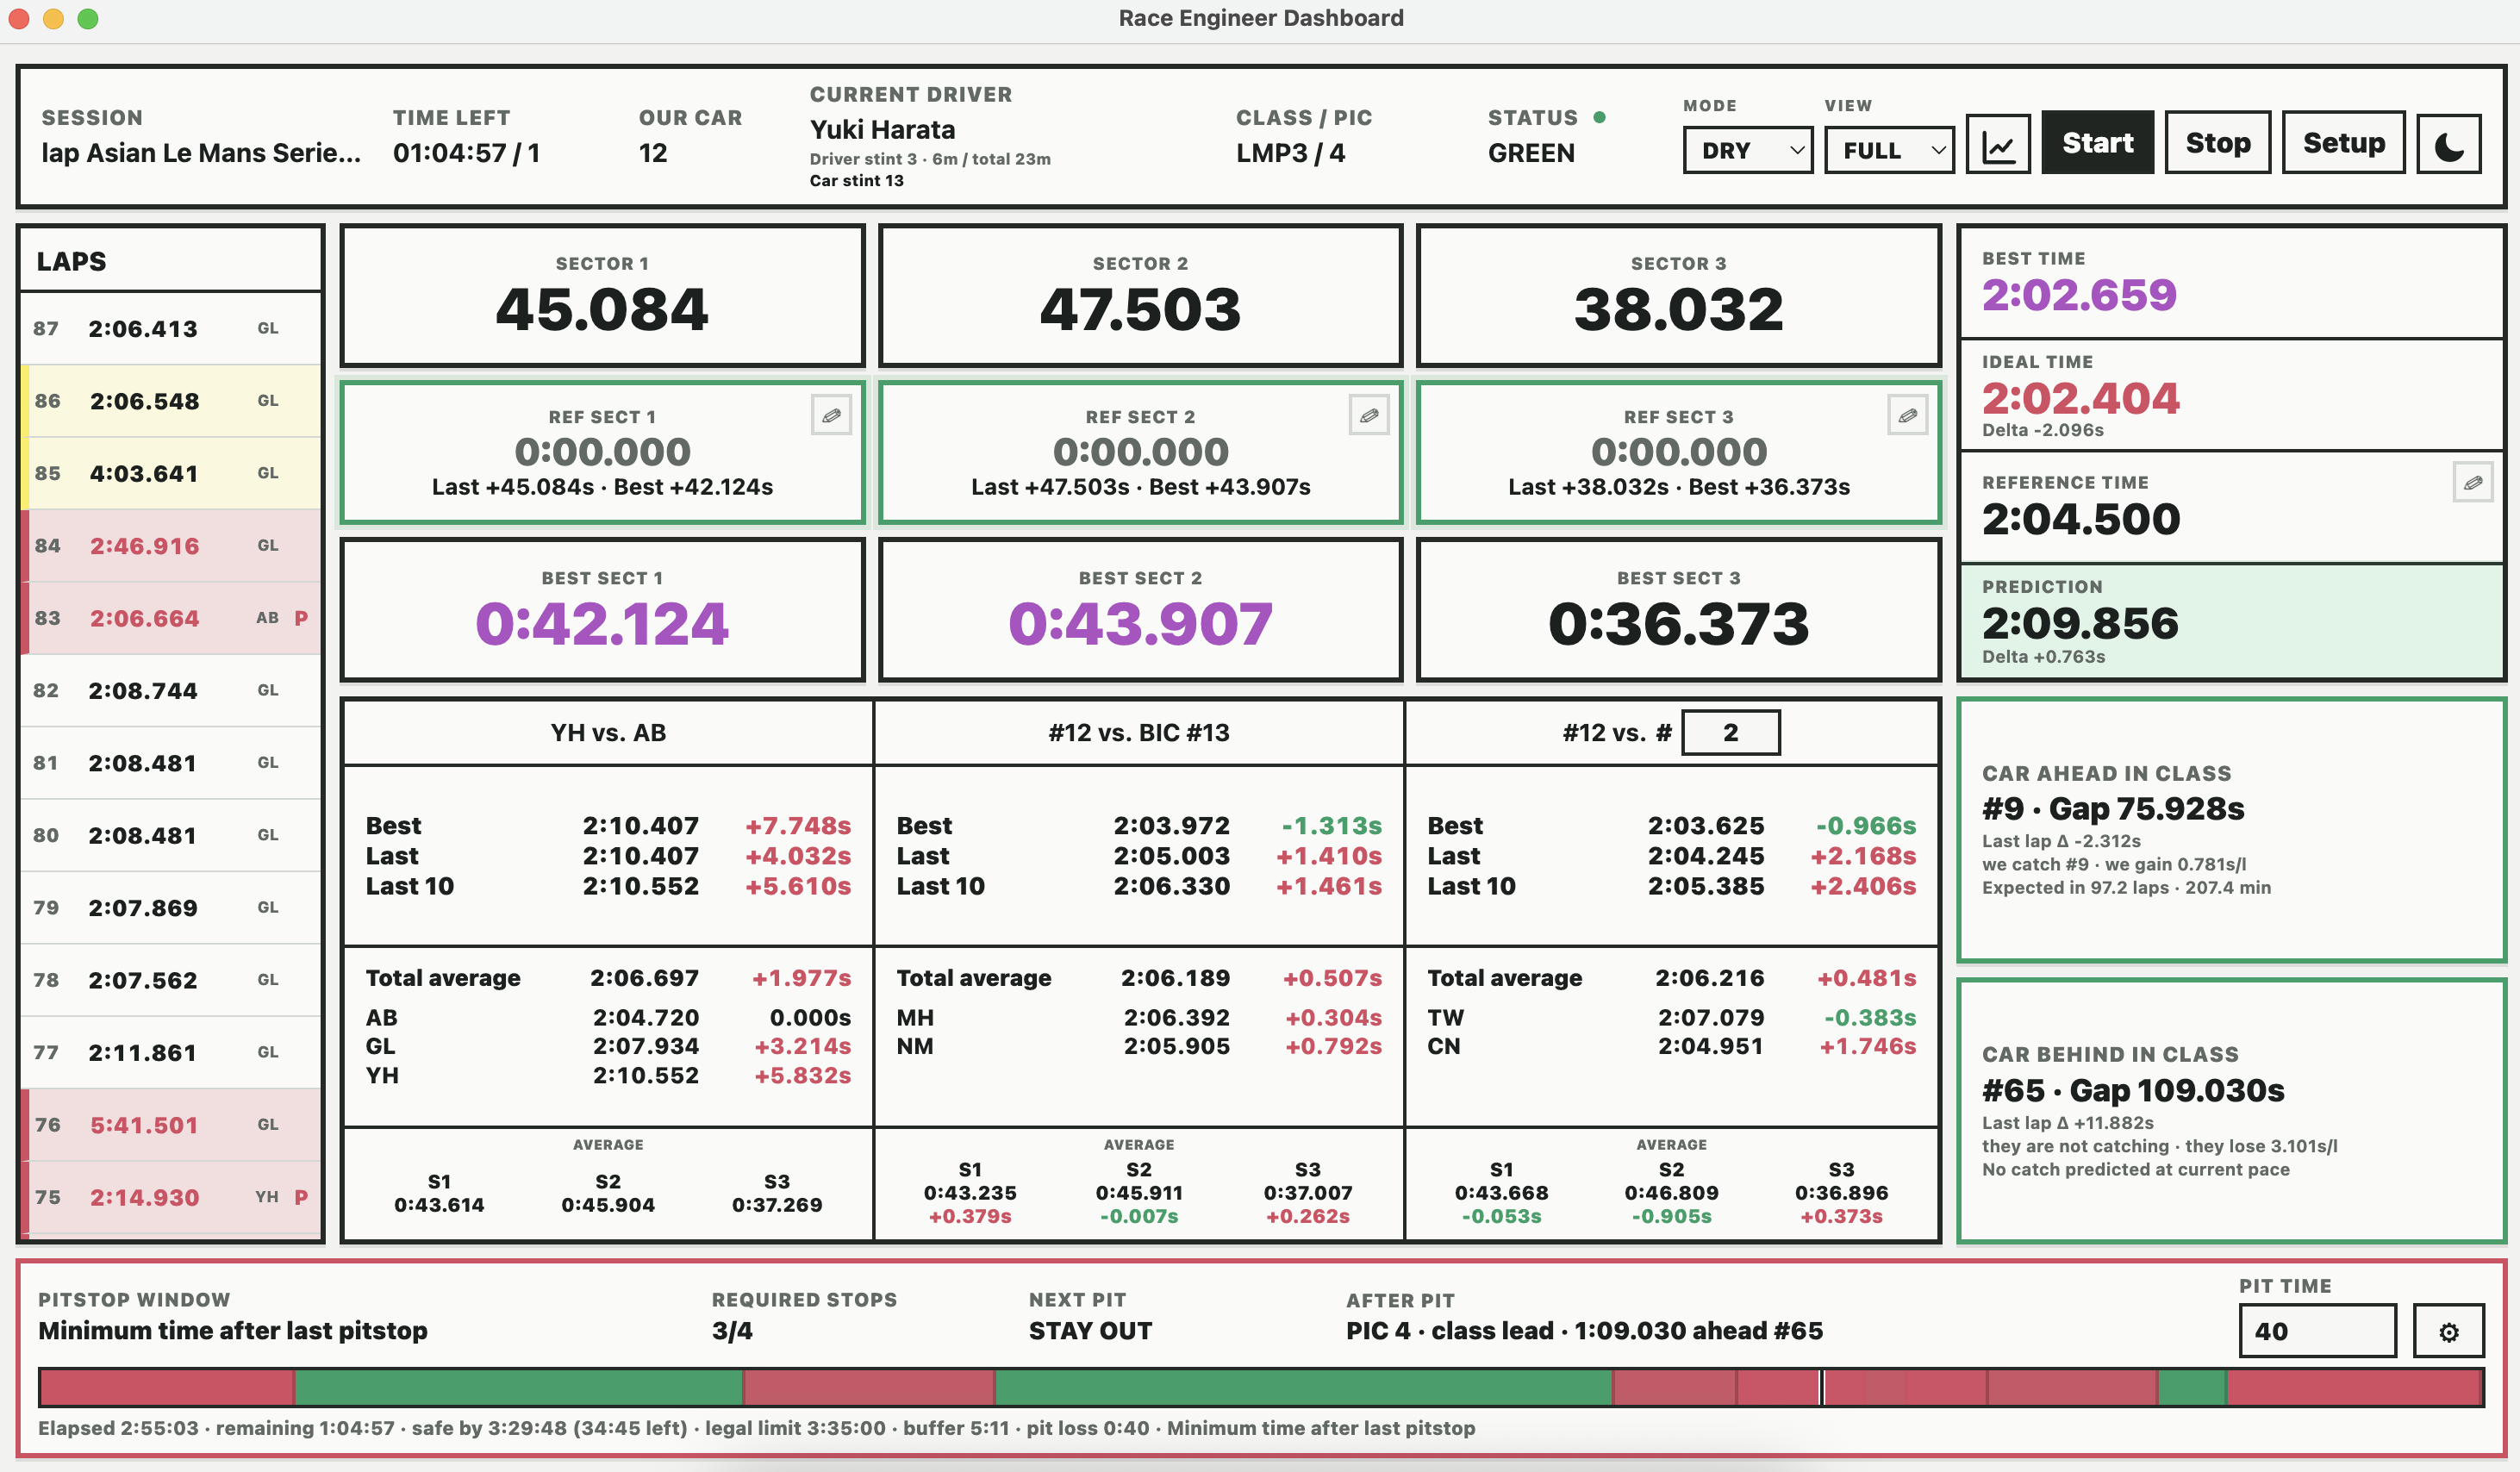
\includegraphics[width=\linewidth]{../figures/final-version.png}

    \small\textbf{Figuur~\thefigure:} Finale versie van het dashboard.
  \end{minipage}\hfill
  
\end{center}



\clearpage
\chapter{Voorbeeld van automatisch gegenereerd raceverslag}
\label{app:spa-race-pdf}

\newcommand{\raceverslagpagina}[1]{%
  \fbox{
\includegraphics[
    page=#1,
    width=0.45\textwidth,
    clip
  ]{../output/pdf/SPA_RACE_CAR_33_ALL_STINTS.pdf}}%
}

\vspace{-0.6em}
\begin{center}
\setlength{\tabcolsep}{2pt}
\renewcommand{\arraystretch}{0.92}
\begin{tabular}{cc}
  \raceverslagpagina{1} & \raceverslagpagina{2} \\
  \raceverslagpagina{3} & \raceverslagpagina{4} \\
  \raceverslagpagina{5} & \raceverslagpagina{6} \\
  \multicolumn{2}{c}{\raceverslagpagina{7}}
\end{tabular}
\end{center}

\clearpage
\chapter*{Afkortingen en begrippen}
\addcontentsline{toc}{chapter}{Afkortingenlijst}

\begingroup
\footnotesize
\setlength{\tabcolsep}{3pt}
\renewcommand{\arraystretch}{0.88}

\section*{Afkortingenlijst}

\begin{tabularx}{\textwidth}{@{}lX@{}}
\toprule
\textbf{Afkorting} & \textbf{Betekenis} \\
\midrule

\multicolumn{2}{@{}l}{\textbf{Applicatie en gegevensverwerking}} \\[0.3em]
CSV   & Comma-Separated Values: tabelformaat voor de opgeslagen timingdata. \\
DOM   & Document Object Model: de programmeerbare structuur van een webpagina. \\
HMI   & Human-Machine Interaction: interactie tussen de gebruiker en de applicatie. \\
IPC   & Inter-Process Communication: communicatie tussen de Electron-processen. \\
UI    & User Interface: de visuele gebruikersinterface van de applicatie. \\

\addlinespace
\multicolumn{2}{@{}l}{\textbf{Motorsport en live timing}} \\[0.3em]
MSTC  & MotorSport Training Center. \\
PIC   & Position in Class: positie van een wagen binnen zijn klasse. \\
BIC   & Best in Class: de best presterende wagen binnen dezelfde klasse. \\
XIC   & Selected Car in Class: een gekozen klassewagen waarmee het team wordt vergeleken. \\
ETA   & Estimated Time of Arrival: geschatte tijd tot een volgend timingpunt. \\
RIS   & Races Information Services: aanbieder van live timingdata. \\
SC    & Safety Car: neutralisatie waarbij het deelnemersveld achter de safety car rijdt. \\
FCY   & Full Course Yellow: neutralisatie waarbij alle wagens hun snelheid beperken. \\

\bottomrule
\end{tabularx}

\vspace{-0.5em}
\section*{Motorsportbegrippen}

\begin{tabularx}{\textwidth}{@{}lX@{}}
\toprule
\textbf{Term} & \textbf{Betekenis} \\
\midrule

Klasse &
Groep wagens met vergelijkbare technische eigenschappen die binnen dezelfde race een afzonderlijk klassement vormen. \\

Sector &
Een deel van het circuit waarvoor afzonderlijk een tussentijd wordt gemeten. \\

Stint &
De aaneengesloten periode waarin een piloot met de wagen rijdt tussen twee pitstops of pilotenwissels. \\

Inlap &
De ronde waarin de wagen aan het einde van de ronde de pitstraat binnenrijdt. \\

Outlap &
De eerste ronde nadat de wagen de pitstraat heeft verlaten. \\

Pitstop window &
Tijdsperiode waarin een verplichte pitstop volgens het wedstrijdreglement geldig mag worden uitgevoerd. \\

Pit loss &
Het geschatte tijdverlies van een pitstop ten opzichte van een wagen die op het circuit blijft rijden. \\

Gap &
Het tijds- of rondeverschil tussen twee wagens. \\

Delta &
Het berekende tijdsverschil tussen twee rondes, sectoren, wagens of piloten. \\

Reference time &
Ingestelde minimale ronde- of sectortijd waarmee actuele en voorspelde tijden worden vergeleken. \\

Ideal lap &
Theoretische rondetijd die ontstaat door de beste geregistreerde sectortijden van dezelfde wagen op te tellen. \\

Track limits &
De toegestane grenzen van het circuit. Een overtreding kan leiden tot het ongeldig verklaren van een rondetijd. \\

Race Control &
Wedstrijdleiding die onder andere vlagstatussen, neutralisaties, straffen en baanveiligheid beheert. \\

Green flag &
Normale racesituatie waarin het circuit vrij is en op wedstrijdsnelheid mag worden gereden. \\

Red flag &
Onderbreking van de sessie omdat verder rijden tijdelijk niet veilig of niet mogelijk is. \\

\bottomrule
\end{tabularx}
\endgroup

\clearpage
\chapter{Stageplan}

\newcommand{\stageplanpagina}[1]{%
  \fbox{\includegraphics[
    page=#1,
    width=0.5\textwidth
  ]{appendices/stageplan_Jeff_Mathieu.pdf}}%
}

\vspace{-0.5em}
\begin{center}
\setlength{\tabcolsep}{3pt}
\begin{tabular}{cc}
  \stageplanpagina{1} & \stageplanpagina{2} \\
  \multicolumn{2}{c}{%
    \fbox{\includegraphics[
      page=3,
      width=0.72\textwidth,
      trim=0 19cm 0 0,
      clip
    ]{appendices/stageplan_Jeff_Mathieu.pdf}}}
\end{tabular}
\end{center}

\clearpage
\chapter{Competenties die ik verwachtte te verbeteren}

\vspace{-0.5em}
\begin{center}
\fbox{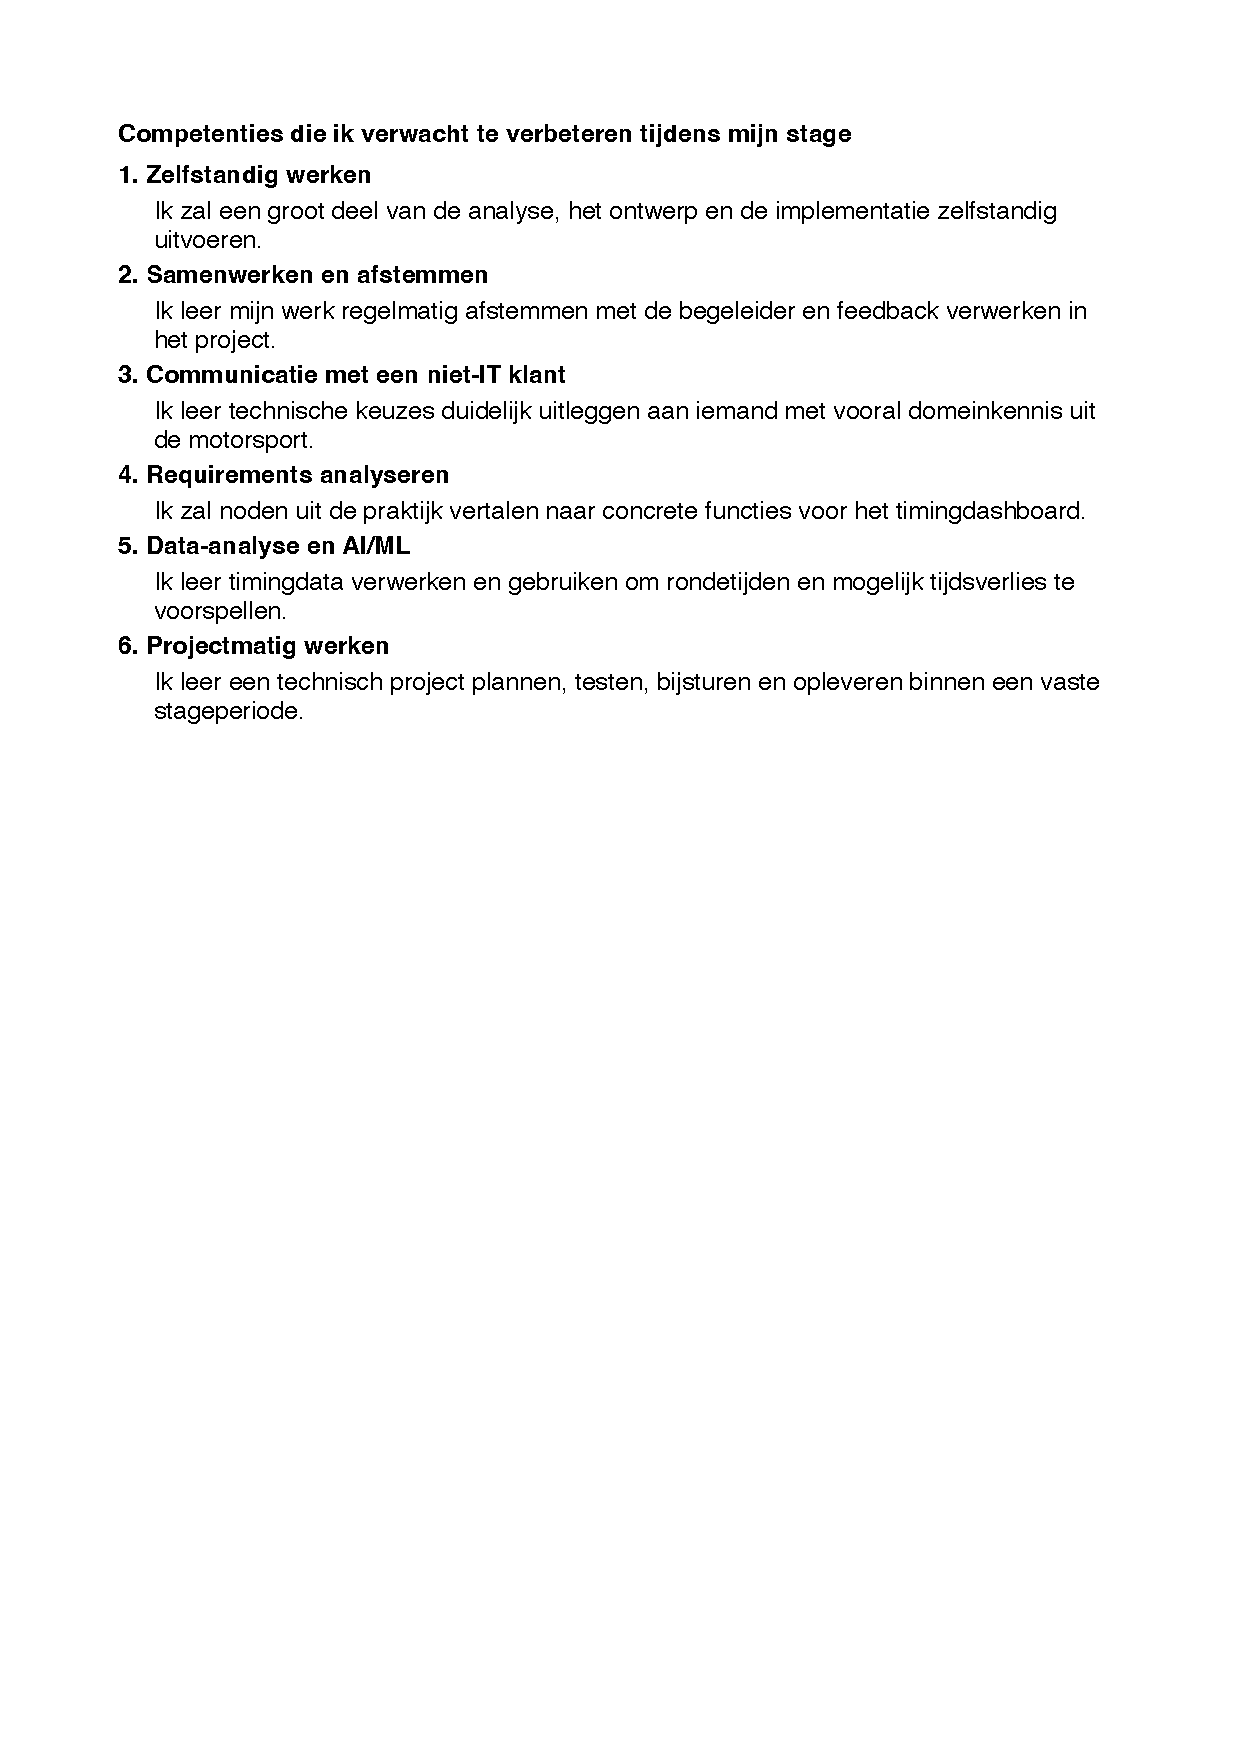
\includegraphics[
  page=1,
  width=0.95\textwidth,
  trim=0 14cm 0 0,
  clip
]{appendices/competenties_Jeff_Mathieu.pdf}}
\end{center}
